\documentclass[paper=a4, fontsize=11pt]{scrartcl} % A4 paper and 11pt font size

\usepackage[T1]{fontenc} % Use 8-bit encoding that has 256 glyphs
\usepackage[english]{babel} % English language/hyphenation
\usepackage{amsmath,amsfonts,amsthm} % Math packages

\usepackage[skip=0pt]{caption}
\usepackage{subcaption}

\usepackage{lipsum} % Used for inserting dummy 'Lorem ipsum' text into the template
\usepackage{graphicx}
\usepackage{sectsty} % Allows customizing section commands
\allsectionsfont{\centering \normalfont\scshape} % Make all sections centered, the default font and small caps

\usepackage{fancyhdr} % Custom headers and footers
\pagestyle{fancyplain} % Makes all pages in the document conform to the custom headers and footers
\fancyhead{} % No page header - if you want one, create it in the same way as the footers below
\fancyfoot[L]{} % Empty left footer
\fancyfoot[C]{} % Empty center footer
\fancyfoot[R]{\thepage} % Page numbering for right footer
\renewcommand{\headrulewidth}{0pt} % Remove header underlines
\renewcommand{\footrulewidth}{0pt} % Remove footer underlines
\setlength{\headheight}{13.6pt} % Customize the height of the header

\iffalse
\numberwithin{equation}{section} % Number equations within sections (i.e. 1.1, 1.2, 2.1, 2.2 instead of 1, 2, 3, 4)
\numberwithin{figure}{section} % Number figures within sections (i.e. 1.1, 1.2, 2.1, 2.2 instead of 1, 2, 3, 4)
\numberwithin{table}{section} % Number tables within sections (i.e. 1.1, 1.2, 2.1, 2.2 instead of 1, 2, 3, 4)
\fi

\setlength\parindent{0pt} % Removes all indentation from paragraphs - comment this line for an assignment with lots of text

% new commands
\newcommand{\horrule}[1]{\rule{\linewidth}{#1}} % Create horizontal rule command with 1 argument of height

\usepackage{listings}
\usepackage{color}
\definecolor{green}{rgb}{0,0.6,0}
\definecolor{gray}{rgb}{0.5,0.5,0.5}
\definecolor{purp}{rgb}{0.58,0,0.82}
\lstset{
  breaklines=true,
  stepnumber=1,
  captionpos=b,
  frame=single,
  numbers=left,
  basicstyle=\footnotesize,
  backgroundcolor=\color{white},
  commentstyle=\color{green},
  numberstyle=\tiny\color{gray},
  keywordstyle=\color{blue},
  stringstyle=\color{purp}
}

\newcommand{\mylisting}[2][]{%
    \lstinputlisting[caption={\texttt{\detokenize{#2}}},#1]{#2}%
}

\definecolor{highlight}{RGB}{248,248,248}


\title{
\normalfont \normalsize
\iffalse
\textsc{Massachusetts Institute of Technology \\ Sloan School of Management, Spring 2016} \\ [25pt] % Your university, school and/or department name(s)
\fi
\horrule{0.5pt} \\[0.4cm] % Thin top horizontal rule
\huge 14.273 Industrial Organization: Problem Set 4 \\ % The assignment title
\horrule{.5pt} \\[0.4cm] % Thick bottom horizontal rule
}

\author{Dave Holtz, Jeremy Yang} % Your name

\date{\normalsize\today} % Today's date or a custom date

\begin{document}
\maketitle
\begin{itemize}
\item[1.] Model setup.\\

Following the notations in Rust \cite{rust1987optimal}, HZ's flow utility is:
\[u(x_t,i_t,\theta_1)+\epsilon_t(i_t) =
\begin{cases}
-RC-c(0,\theta_1)+\epsilon_t(1) & i_t = 1\\
-c(x_t,\theta_1)+\epsilon_t(0) & i_t=0
\end{cases}\]
where $RC$ is the replacement cost, $x_t$ is the observed state variable for mileage, $c(\cdot)$ is cost function and $i_t$ is the decision to replace engine and $\epsilon_t(\cdot)$ is action specific and type I extreme value distributed structural error (or unobserved state variable).\\

The state transition probability is given by:
\[\theta_{3j} = \mathbb{P}(x_{t+1}=x_t+j|x_t,i_t=0)\]
$j \in \{0,1,2\}$ and if $i_{t}=1$ then $x_{t+1}=0$ with probability 1.\\

HZ chooses $i_t$ in every period $t$ to maximize an infinite sum of discounted flow utilities. The maximal value is defined as the value function (suppress the dependency on $\theta_1, \theta_3$):
\[V(x_1,\epsilon_1) := \text{max}_{i_t, t\in\{1,2,..\}}\ \mathbb{E}[\sum_{t=1}^\infty \beta^{t-1} (u(x_t,i_t,\theta_1)+\epsilon_t(i_t))]\]

Rewrite the value function as in the Bellman optimality form:
\[V(x_t, \epsilon_t) = \text{max}_{i_t} \ (u(x_t,i_t,\theta_1)+\epsilon_t(i_t)) + \beta \mathbb{E}[V(x_{t+1},\epsilon_{t+1})|x_t, i_t]\]
where the expectation is with respect to (conditional) state transition probability of both $x$ and $\epsilon$, see Rust \cite{rust1987optimal} equation (4.5). The Bellman equation breaks the dynamic optimization problem into an infinite series of static choices.


\item[2.]
\begin{itemize}
\item[(1)] The choice specific value function can be derived by plugging a specific action into the value function:
\[\tilde{V}(x_t,\epsilon_t,i_t)=
\begin{cases}
-RC-c(0,\theta_1)+\epsilon_t(1) + \beta \mathbb{E}[V(x_{t+1},\epsilon_{t+1})|x_t, i_t=1] \\
-c(x_t,\theta_1)+\epsilon_t(0) + \beta \mathbb{E}[V(x_{t+1},\epsilon_{t+1})|x_t, i_t=0]
\end{cases}\]
\[V(x_t,\epsilon_t) = \text{max}\{\tilde{V}(x_t,\epsilon_t,1),\tilde{V}(x_t,\epsilon_t,0)\}\]
HZ's decision is about trading off the total (future) cost of maintaining an old engine and the lump sum cost of replacing to a new one. The time to replace is the stopping time in this problem, so it can be thought as an optimal stopping time problem where the optimal policy is characterized by a cutoff in $x$, HZ would choose to replace the engine if $x$ is above that threshold (the threshold depends on realized value of $\epsilon$).

\item[(2)] It's clear from 2 (1) that the optimal stopping rule is:
\begin{align*}
&-RC-c(0,\theta_1)+\epsilon_t(1) + \beta \mathbb{E}[V(x_{t+1},\epsilon_{t+1})|x_t, i_t=1] >\\
&-c(x_t,\theta_1)+\epsilon_t(0) + \beta \mathbb{E}[V(x_{t+1},\epsilon_{t+1})|x_t, i_t=0]
\end{align*}
or,
\[\tilde{V}(x_t,\epsilon_t,1) > \tilde{V}(x_t,\epsilon_t,0)\]
therefore, because the errors are type I extreme value distributed:
\[\mathbb{P}(i_t=1|x_t) = \frac{\text{exp}(u(x_t,1,\theta_1)+\beta \mathbb{E}[V_{t+1}|x_t, i_t=1])}{\sum_{k=\{0,1\}}\text{exp}(u(x_t,k,\theta_1)+\beta \mathbb{E}[V_{t+1}|x_t, i_t=k]}\tag{2.1}\]
where $u(x_t,i_t,\theta_1)$ is defined in 1 and for convenience:
\[V_{t+1} :=V(x_{t+1},\epsilon_{t+1})\]

\item[(3)]
For discrete $x$, under the assumption that the errors are type I extreme value distributed, we have (Rust \cite{rust1987optimal} equation (4.14)):
\[EV(x,i) = \sum_y \text{log} \{\sum_{j} \text{exp}[u(y,j)+\beta EV(y,j)]\}\cdot p(y|x,i)\tag{2.2}\]
where
\[EV(x,i) := \mathbb{E}[V_{t+1}|x_t,i_t]\]
and $x, i$ are the state and choice of current period and $y,j$ are the state and choice of the next period. Also note that here the transition probability does not depend on $x_t$ but only on $j$ (or $\Delta x$). To compute expected value function, we first need to estimate transition probability from the data, this can be done simply by counting:
\[\hat{\theta}_{30} = \frac{\sum_{b}\sum_{t} 1_{\{x_{bt+1}-x_{bt}=0, i_{bt}=0\}}}{\sum_{b}\sum_{t} 1_{\{i_{bt}=0\}}}\]
\[\hat{\theta}_{31} = \frac{\sum_{b}\sum_{t} 1_{\{x_{bt+1}-x_{bt}=1, i_{bt}=0\}}}{\sum_{b}\sum_{t} 1_{\{i_{bt}=0\}}}\]
\[\hat{\theta}_{32} = \frac{\sum_{b}\sum_{t} 1_{\{x_{bt+1}-x_{bt}=2, i_{bt}=0\}}}{\sum_{b}\sum_{t} 1_{\{i_{bt}=0\}}}\]
we compute the expected value function in the inner loop of the nested fixed point algorithm (holding the value of $\theta$ fixed), we first guess the initial values of $EV(x,i)$ for all possible values of $x,i$ and use the equation (2.2) to iterate expected value function until it converges. The criterion is:
\[\text{max}_{x,i}|EV^{T+1}(x,i)-EV^T(x,i)|<\eta\]

The plot for $x=1-30$ at the true value of parameters are shown in Figure \ref{fig:ev_plot}'s left panel. The provided EV values for the Rust dataset are provided in Figure \ref{fig:ev_plot}'s right panel. The two match well, suggesting that our implementation is working as expected. There is some strange behavior in the tail (for mileage $\in$ (29, 30). We suspect this is truncation error from not having data for higher states.

\begin{figure}[ht!]
\centering
	\begin{minipage}[b]{.46\linewidth}
		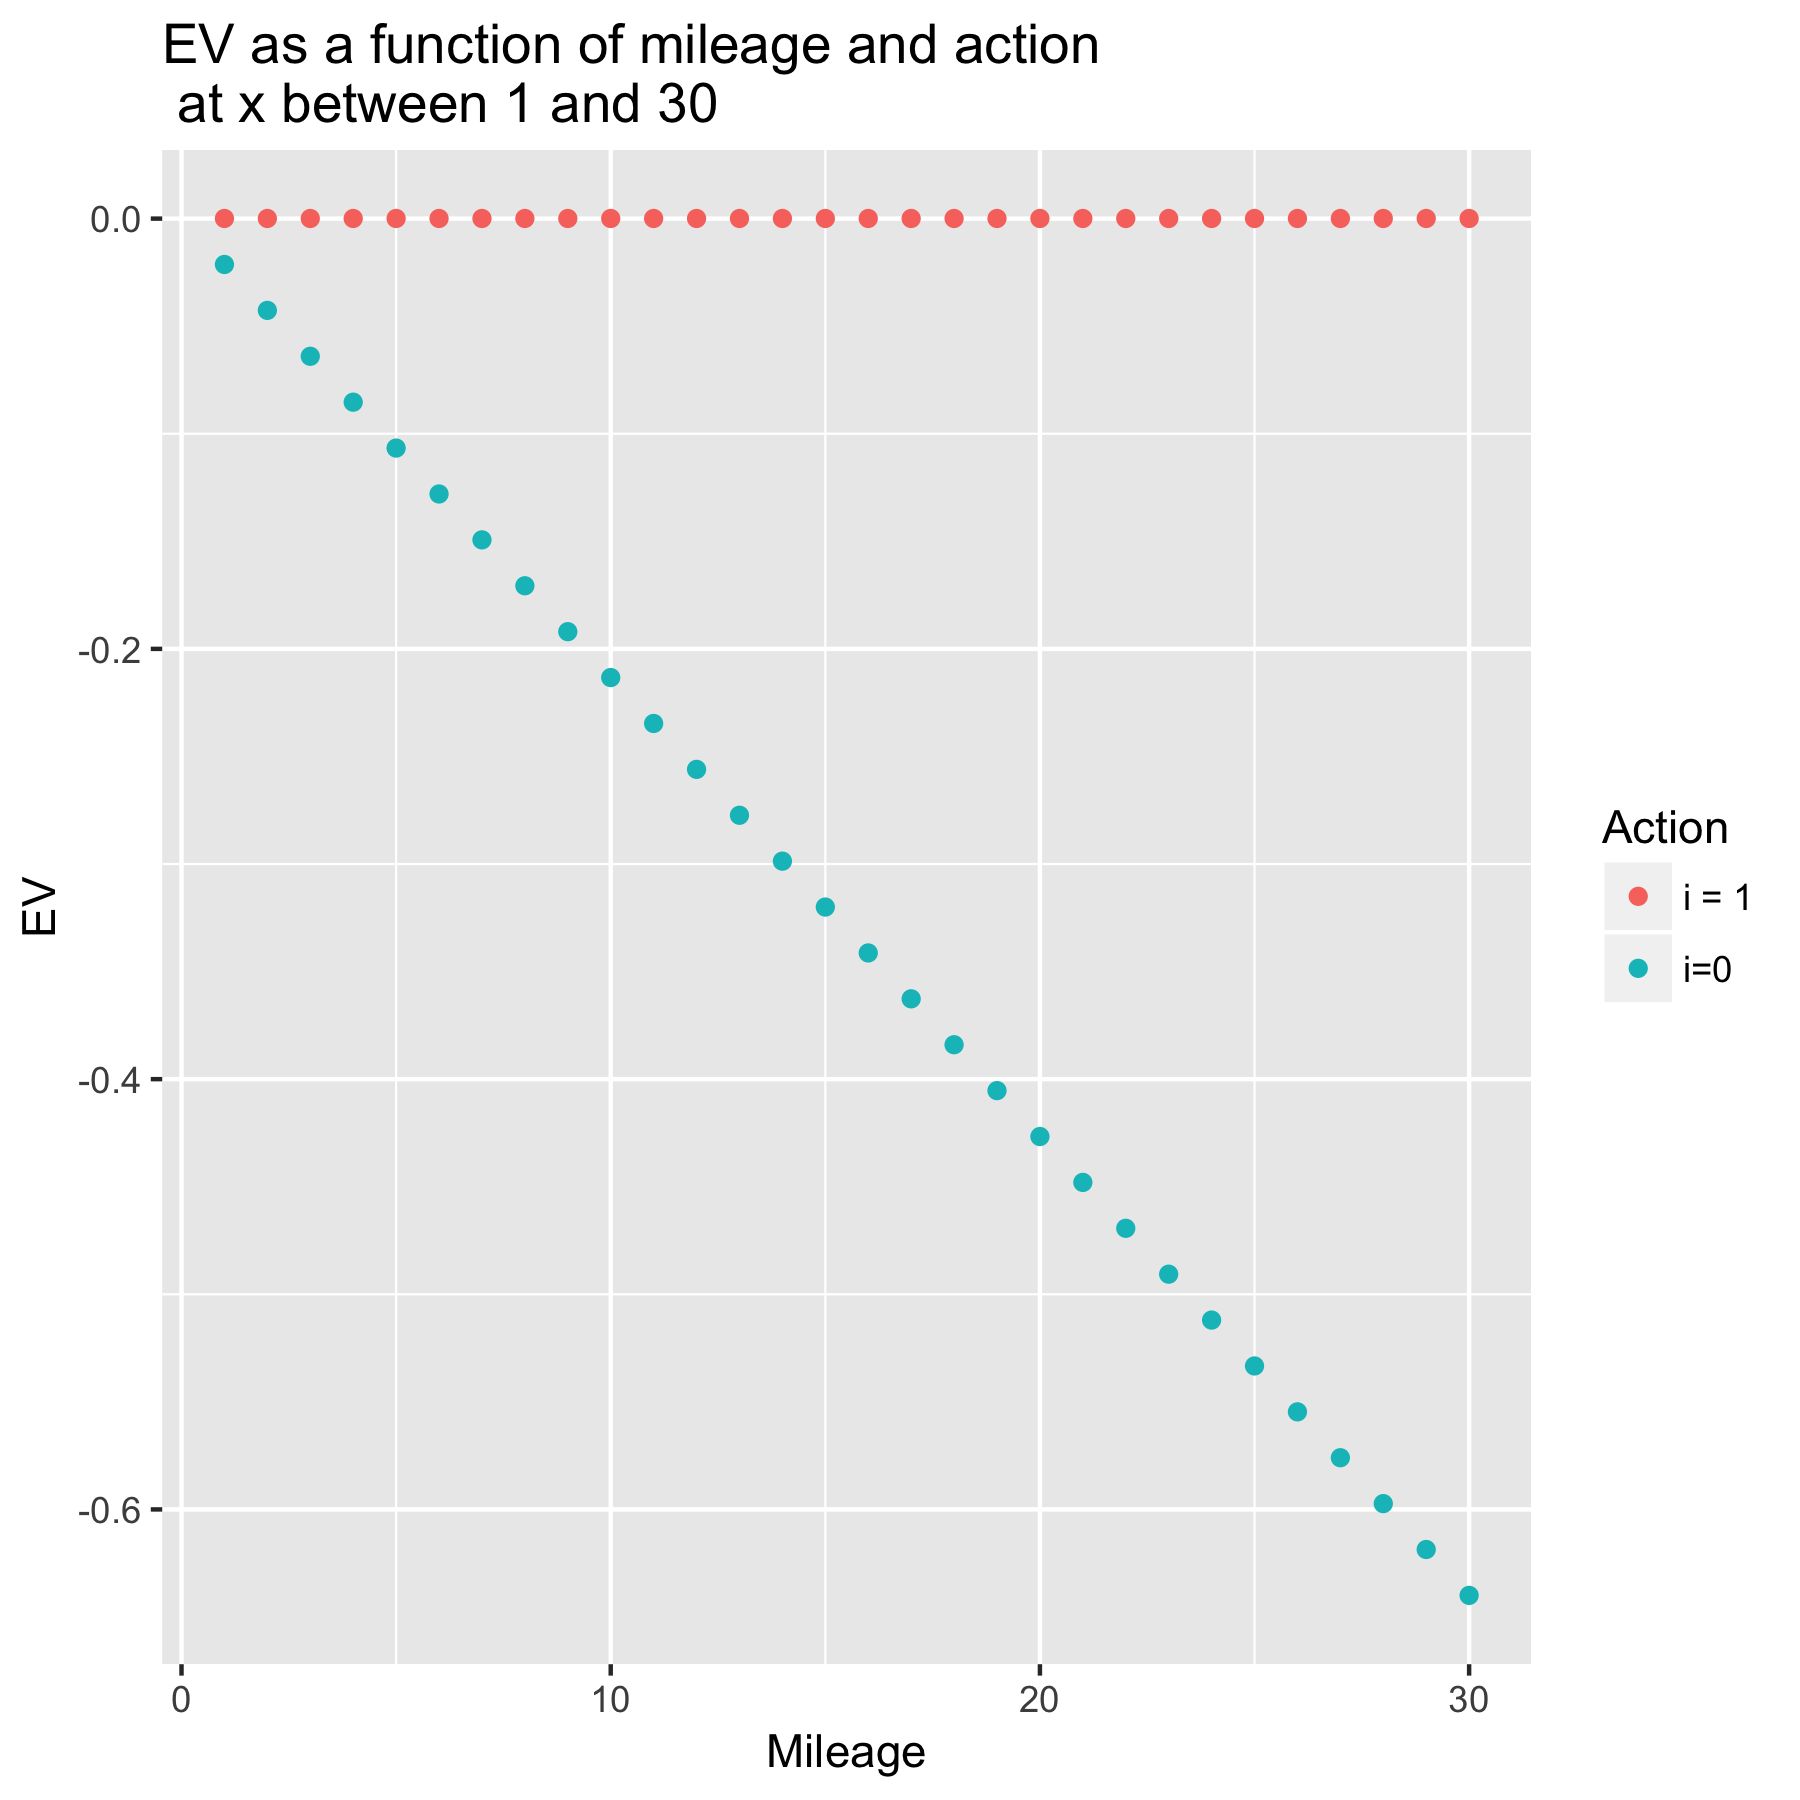
\includegraphics[scale=.1]{ev_plot.png}
	\end{minipage}
	\begin{minipage}[b]{.46\linewidth}
		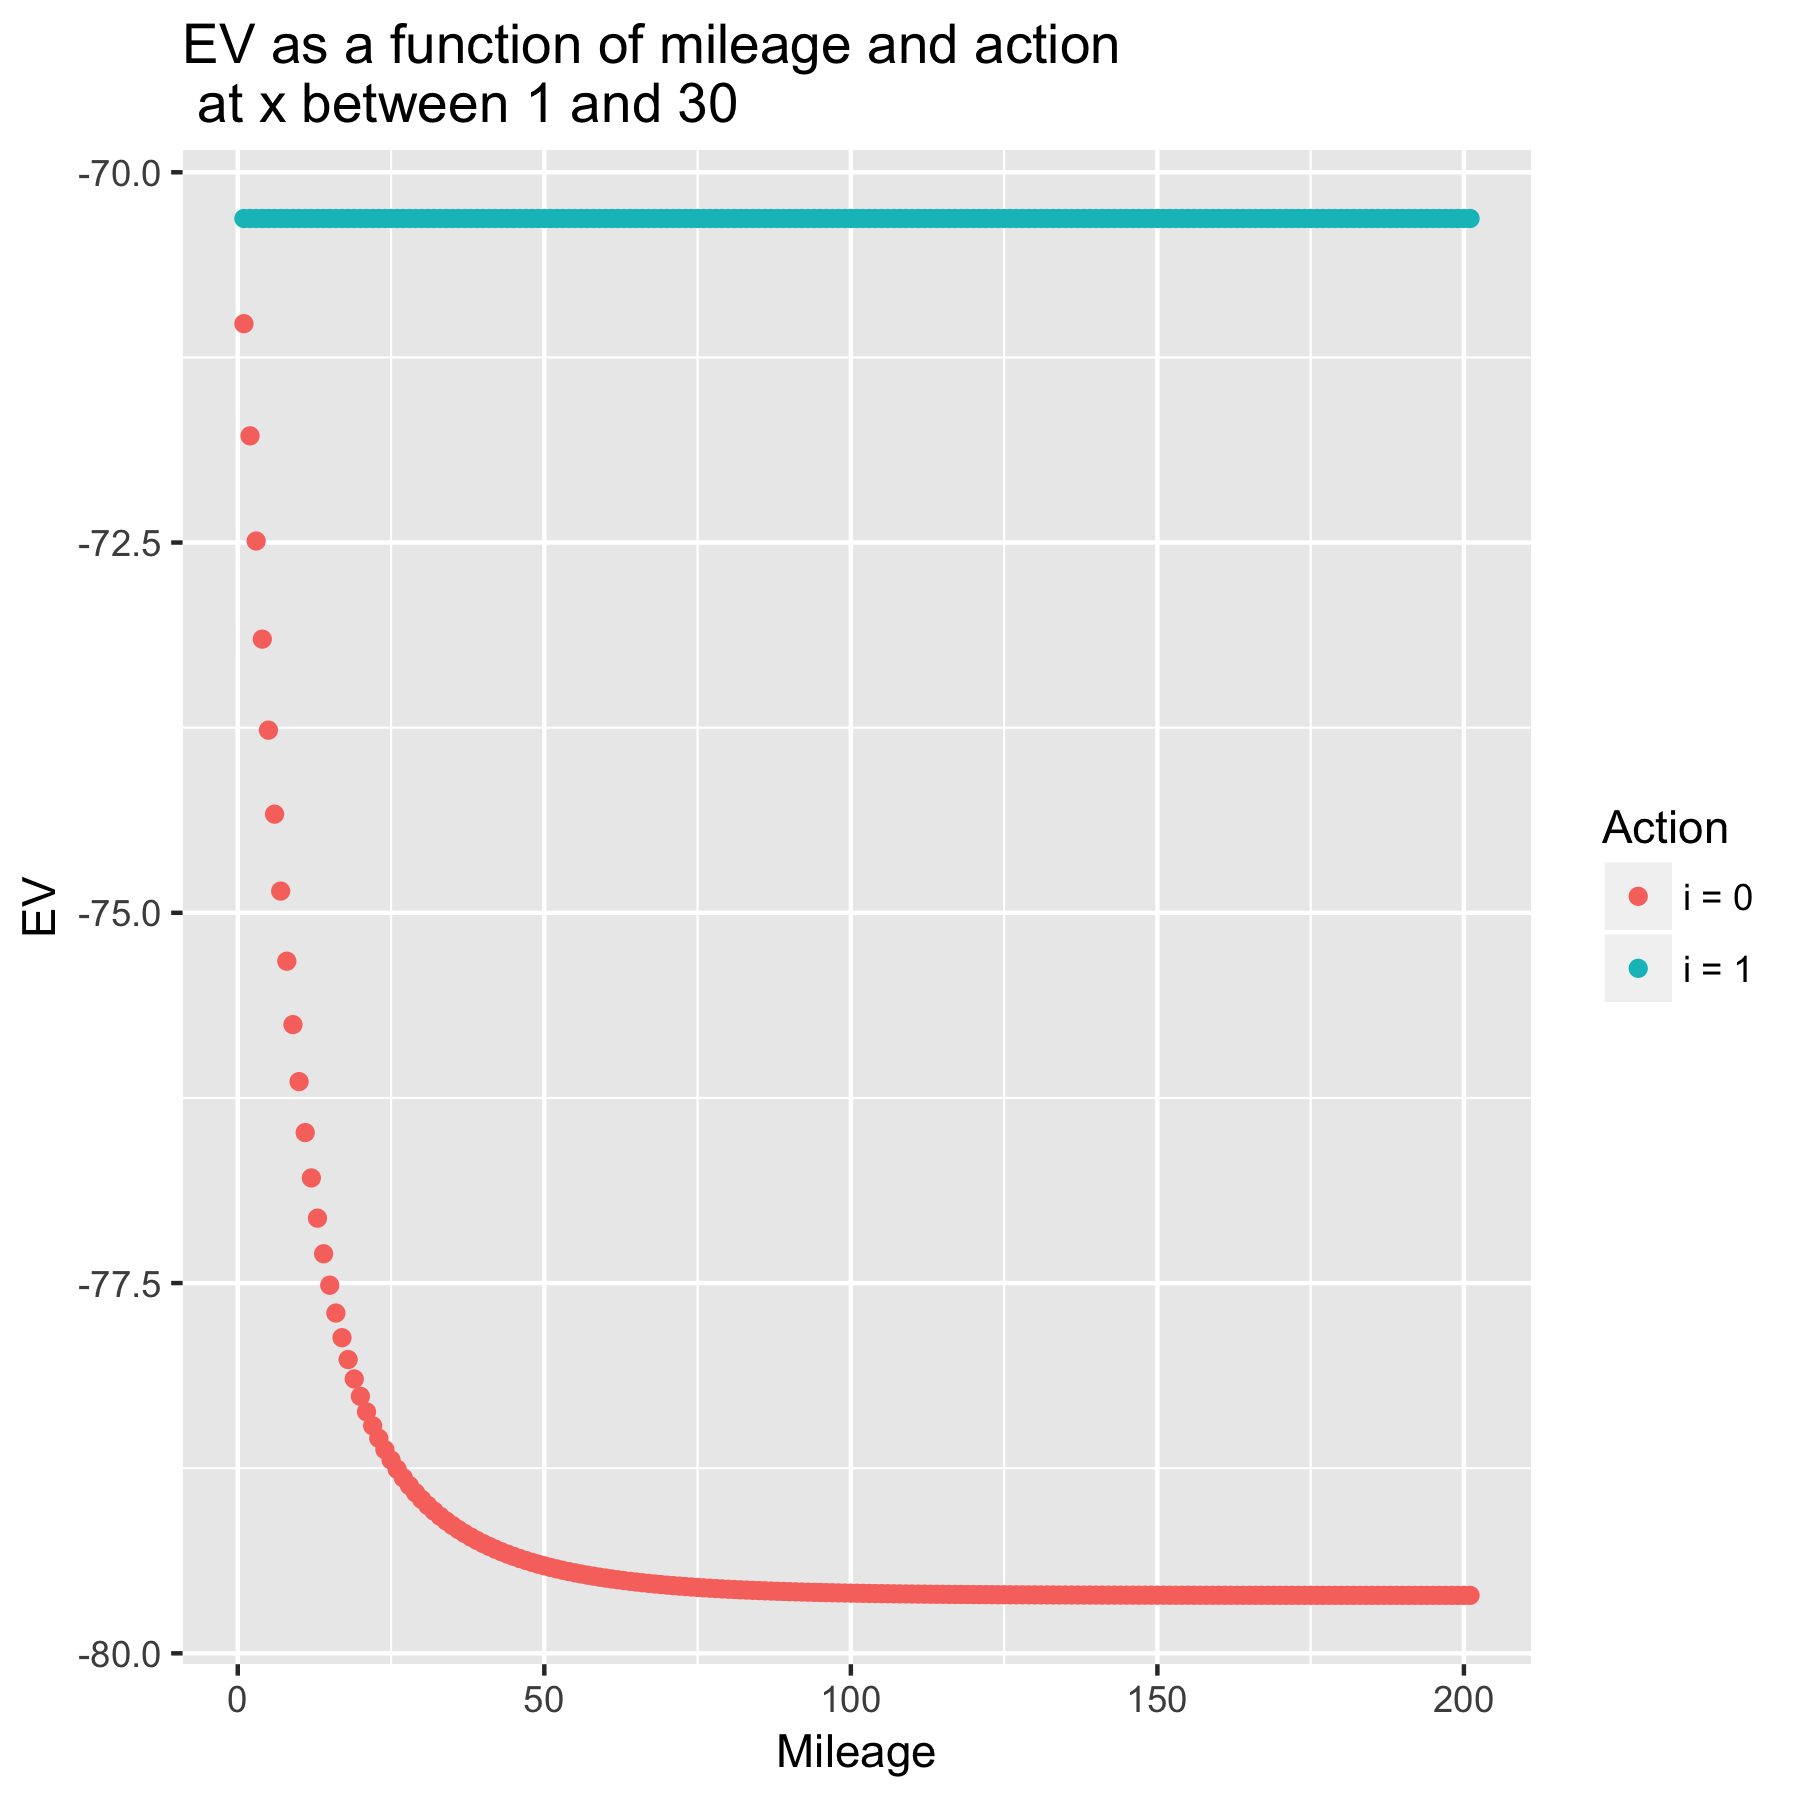
\includegraphics[scale=.1]{ev_plot_rust.png}
	\end{minipage}
\caption{Expected Value Function for $i = 0$ and $i = 1$. Left panel shows results using iterative method, right panel shows provided Rust results.}
\label{fig:ev_plot}
\end{figure}

\item[(4)]

The provided dataset contains mileage and engine replacement information for 100 buses over 1,000 periods. The table below shows the mean mileage, maximum mileage, minimum mileage, standard deviation of the mileage, the average mileage at engine replacement across all buses and periods, and the average number of engine replacements for a particular bus over the 1,000 periods.

\begin{center}
\begin{tabular}{r | r | r | r | r | r}
\hline
avg miles & max miles & min miles & s.d. miles & avg replace miles & avg replacements\\
8.245 & 33.000 & 0.000 & 5.709 & 15.953 & 52.980 \\
\hline
\end{tabular}
\end{center}

We might also be interested in understanding how each of these summary statistics vary across buses. For instance, maybe some buses have their engines replaced much more often. In order to study this, Figure \ref{fig:summary_statistics} shows the distributions of average mileage, maximum mileage, s.d. mileage, avg miles at replacement, and number of replacements across the 100 buses in the sample. In general, these distributions are quite concentrated, suggesting that there are not systematic differences across buses.

The final, bottom right plot in \ref{fig:summary_statistics} also shows the empirically observed conditional choice probability as a function of state (mileage) that Harold Zurcher actually acts on. At a high level, Zurcher's has to make the investment decision of when to replace a given bus's engine. The mean replacement mileage plot suggests that on average he replaces a bus's engine after about 80,000 miles. The conditional choice probability plot suggests that the likelihood he increases the engine is practically zero until the bus hits 50,000 miles, after which the probability that the bus has its engine replaced climbs quickly. By the time a bus has 150,000 miles on it, it has a 50\% probability of having its engine changed in a given time period.

\begin{figure}
	\centering
	\begin{minipage}[b]{.48\linewidth}
		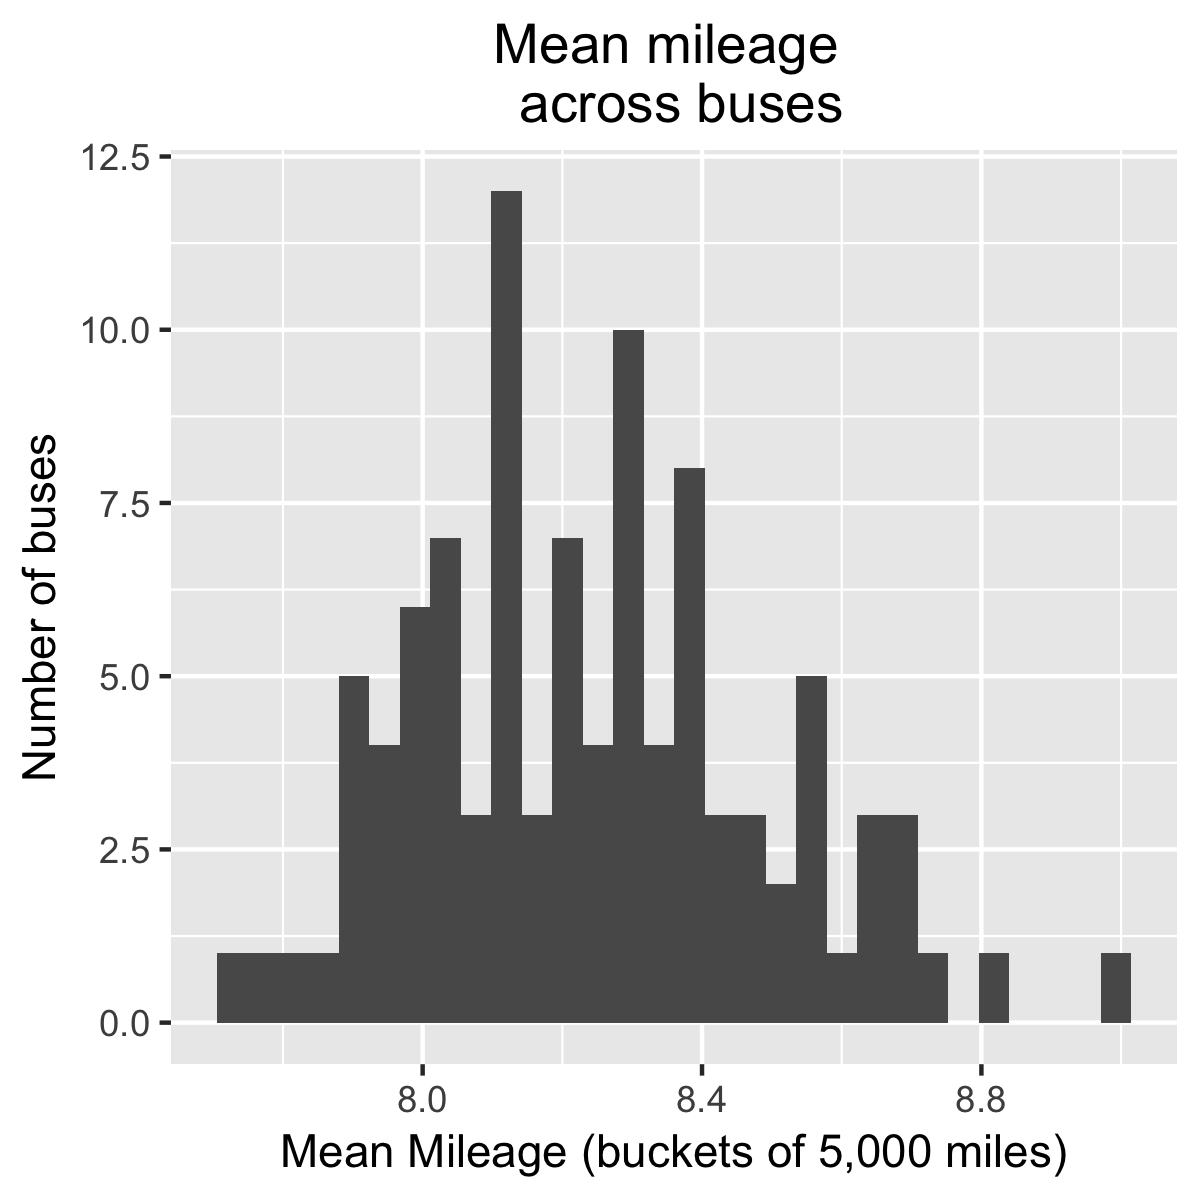
\includegraphics[scale=.15]{mean_mileage_plot.png}
	\end{minipage}
	\begin{minipage}[b]{.48\linewidth}
		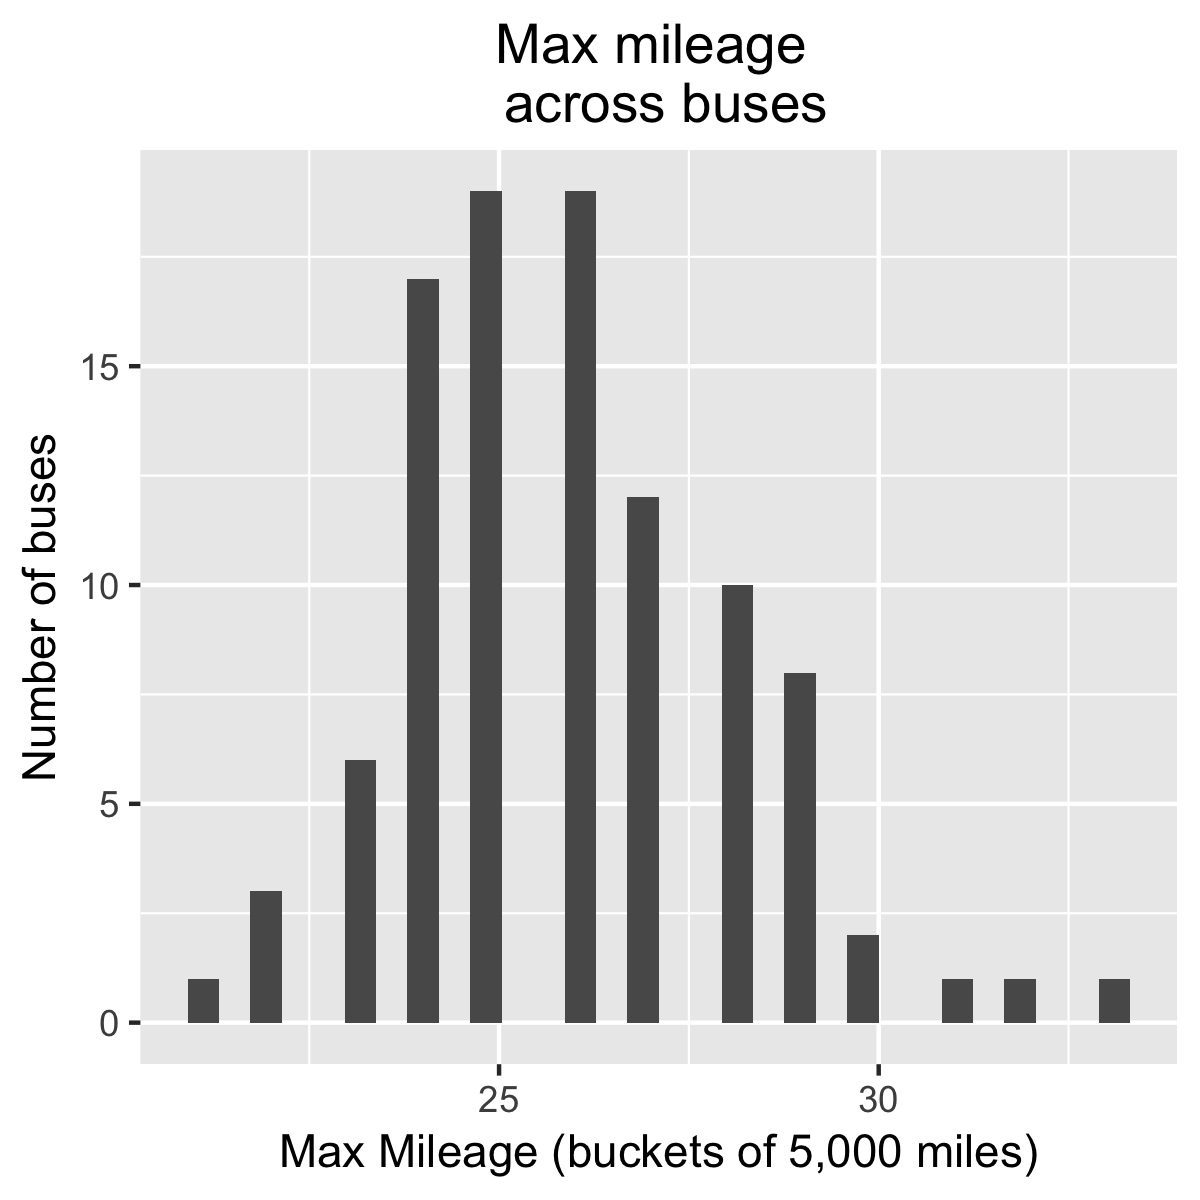
\includegraphics[scale=.15]{max_mileage_plot.png}
	\end{minipage}
	\begin{minipage}[b]{.48\linewidth}
	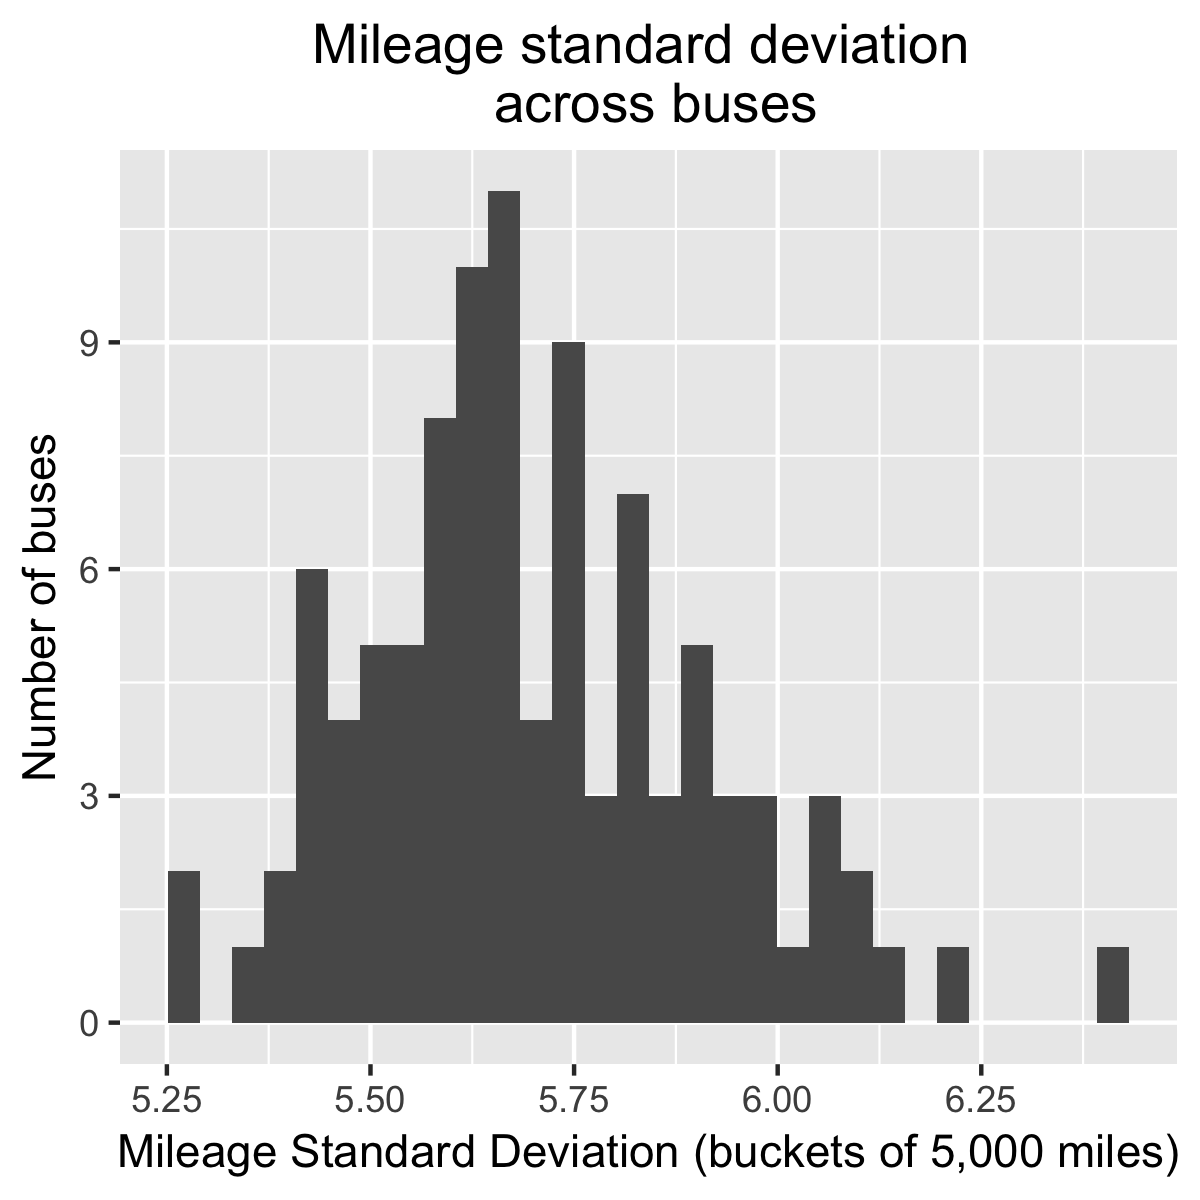
\includegraphics[scale=.15]{sd_mileage_plot.png}
	\end{minipage}
	\begin{minipage}[b]{.48\linewidth}
	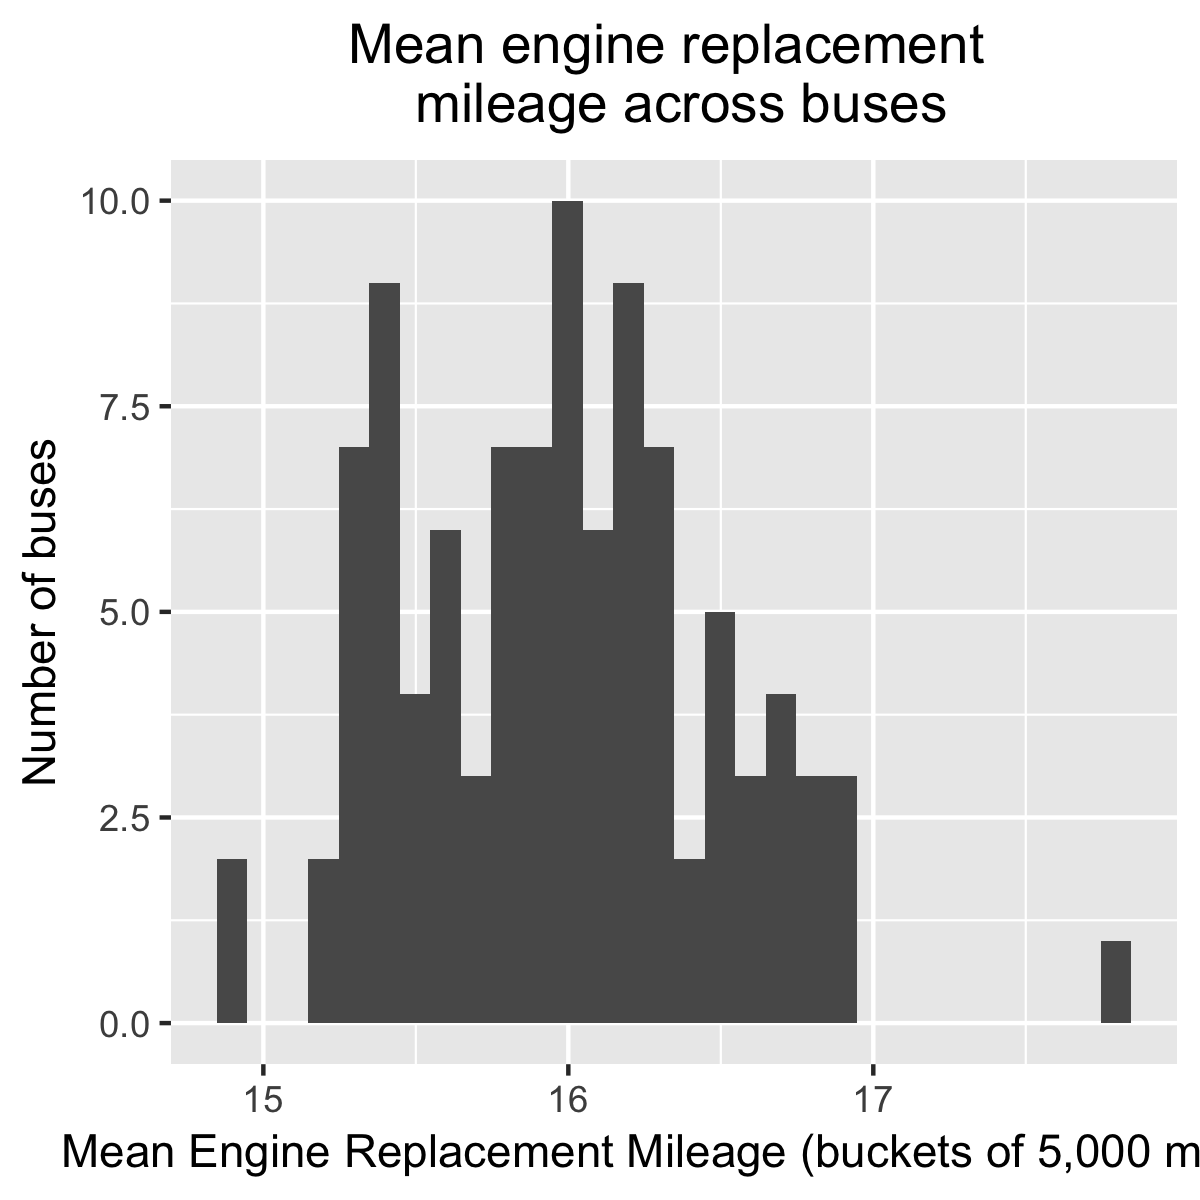
\includegraphics[scale=.15]{time_to_engine_replacement_plot.png}
	\end{minipage}
		\begin{minipage}[b]{.48\linewidth}
	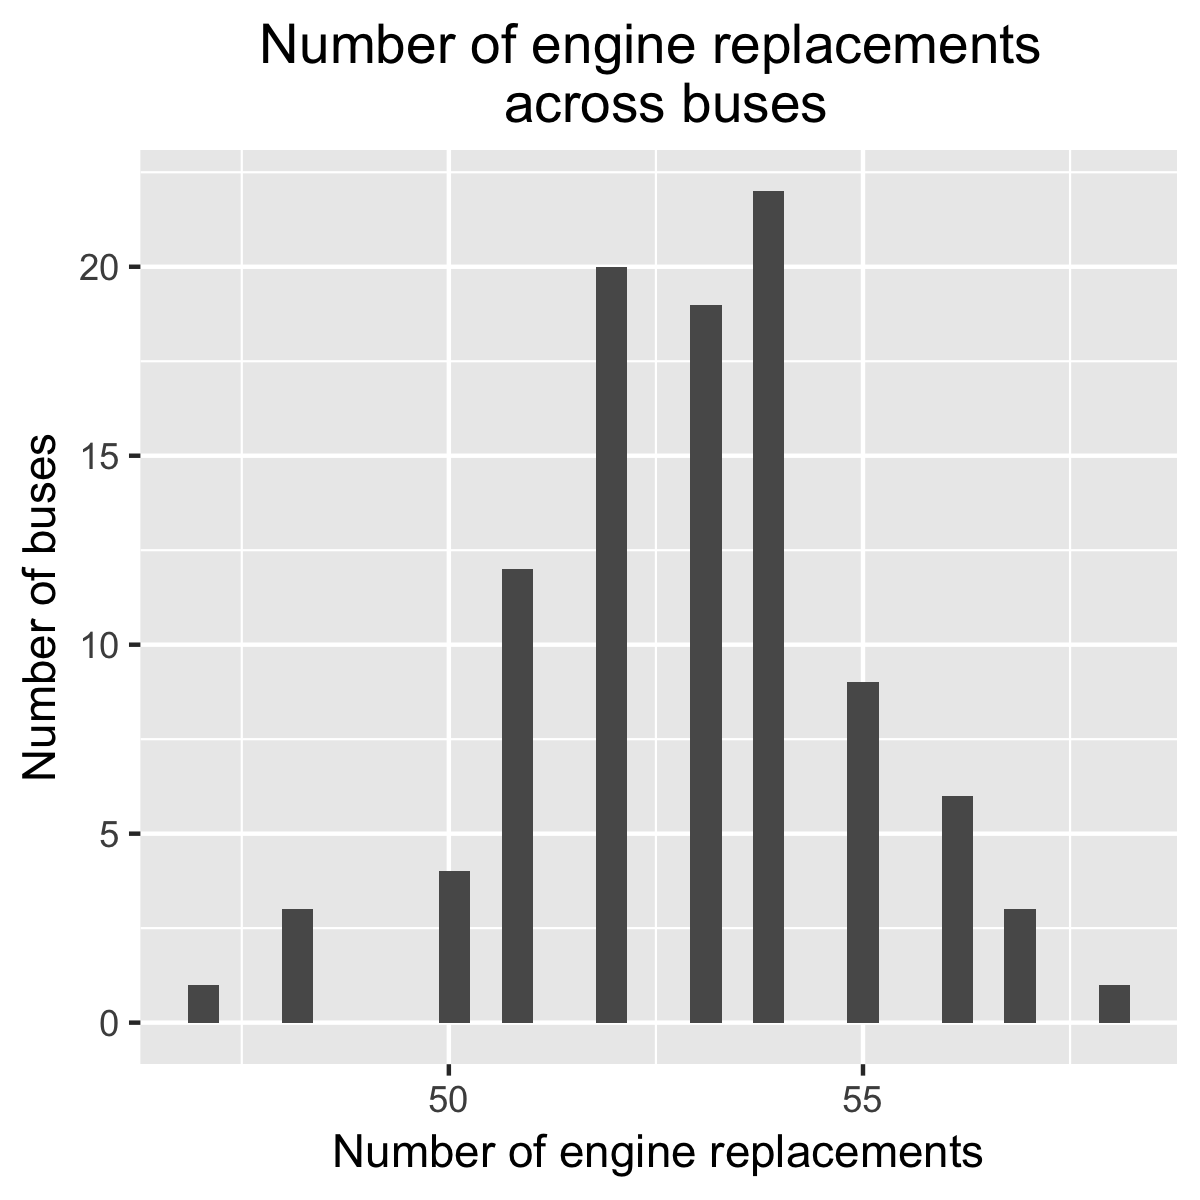
\includegraphics[scale=.15]{replacements_plot.png}
	\end{minipage}
	\begin{minipage}[b]{.48\linewidth}
	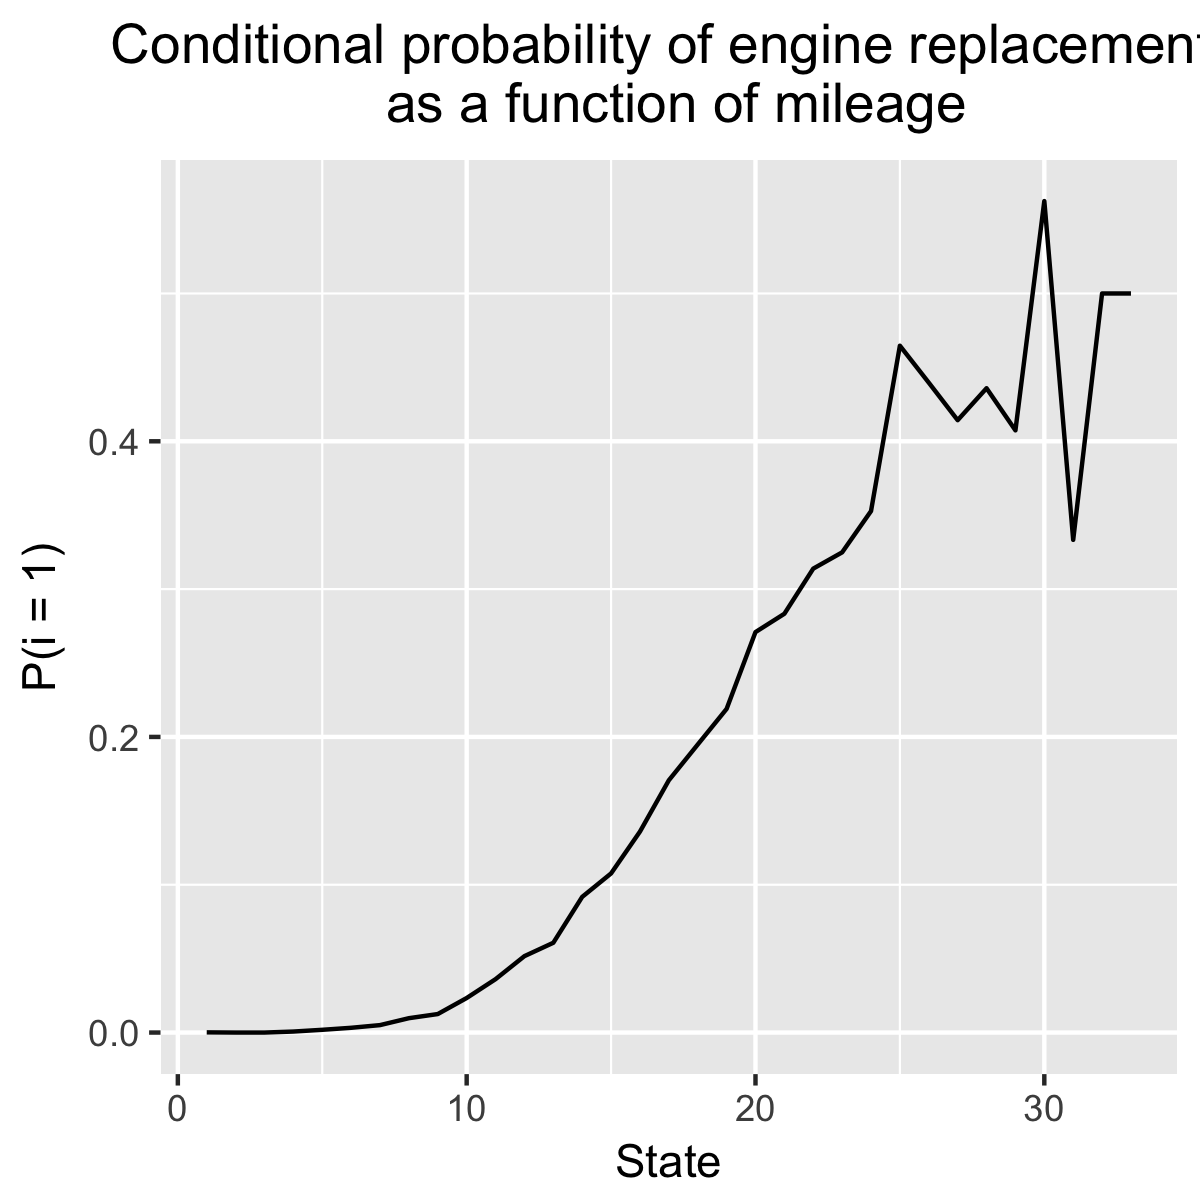
\includegraphics[scale=.15]{ccp_plot.png}
	\end{minipage}
	\caption{Distribution of various summary statistics across buses, as well as the empirical conditional choice probability for Zurcher.}
	\label{fig:summary_statistics}
\end{figure}

\end{itemize}

\item[3.]
\begin{itemize}
\item[(1)] In the outer loop we search over a grid of values for $(\theta_1, \beta, RC)$, and compute the log likelihood function:
\[\text{log}L = \sum_{b} \{\sum_{t} \text{log} \mathbb{P}(i_{bt}|x_{bt}) + \sum_t \text{log} \mathbb{P}(x_{bt}|x_{bt-1},i_{t-1})\}\]
where $b$ indexes for bus and $t$ indexes for time period. We compute a log likelihood for each combination of values for $(\theta_1, \beta, RC)$ and choose the set of parameters that maximizes the log-likelihood of the data. The maximum likelihood parameters obtained with the Rust \cite{rust1987optimal} method are:

\begin{eqnarray*}
\theta_1 & = 0.05 \\
\beta & = 0.99 \\
RC & = 10
\end{eqnarray*}

The maximum-likelihood parameters that we obtain using the Rust method are exactly identical to the ``true" parameters.

\item[(2)] In Hotz-Miller's \cite{hotz1993conditional} approach, we will estimate the choice specific value function (as opposed to the expected value function as in Rust). We start by noting that conditional choice probability is observed directly from the data:
\[\hat{\mathbb{P}}(i=1|x) = \frac{\sum_{b}\sum_{t} 1_{\{i_{bt}=1, x_{bt}=x\}}}{\sum_{b}\sum_{t} 1_{\{x_{bt}=x\}}}\]
The choice-specific value function (minus the structural error, and suppressing the dependency on $\theta_1, \theta_3$) can be presented recursively in the following form:
\[\tilde{V}(x_t,i_t) = u(x_t,i_t)+\beta\mathbb{E}_{x_{t+1}}[\mathbb{E}_{i_{t+1}}[\mathbb{E}_{\epsilon_{t+1}}[u(x_{t+1},i_{t+1})+\epsilon_{t+1}+\beta(\cdot\cdot\cdot)|i_{t+1},x_{t+1}]|x_{t+1}]|x_t,i_t]\]
where $(\cdot\cdot\cdot)$ represents higher (two and above) period forward expectations. In principle it's an infinite loop but in practice we need to stop at some $T$, for example, when $T=2$, $(\cdot\cdot\cdot)$ simplifies to:
\[(\cdot\cdot\cdot) = \mathbb{E}_{x_{t+2}}[\mathbb{E}_{i_{t+2}}[\mathbb{E}_{\epsilon_{t+2}}[u(x_{t+2},i_{t+2})+\epsilon_{t+2}|i_{t+2},x_{t+2}]|x_{t+2}]|x_{t+1},i_{t+1}]\]
For simplicity, in the code we use one-period forward simulation where:
\[\tilde{V}(x_t,i_t) = u(x_t,i_t)+\beta\mathbb{E}_{x_{t+1}}[\mathbb{E}_{i_{t+1}}[\mathbb{E}_{\epsilon_{t+1}}[u(x_{t+1},i_{t+1})+\epsilon_{t+1}|i_{t+1},x_{t+1}]|x_{t+1}]|x_t,i_t]\]
it is estimated as:
\[\hat{\tilde{V}}(x_t,i_t) = \frac{1}{S} \sum_{s} [u(x_t,i_t)+\beta[u(x^s_{t+1},i^s_{t+1})+\gamma -\text{log}(\hat{\mathbb{P}}(i^s_{t+1}|x^s_{t+1}))]]\]
where $x^s_{t+1}$ is drawn from the transition probability $\hat{\theta}_{30}, \hat{\theta}_{31}, \hat{\theta}_{32}$, and $i^s_{t+1}$ is drawn from $\hat{\mathbb{P}}(i|x)$, $\gamma$ is the Euler's constant. 

We only go one period forward because we only observe data for states up to $x_t = 33$. It is possible for larger $T$ that we would encounter a state that is not in our dataset. When this occurs, its unclear what value should be used as the conditional choice probability. While we avoid this issue by setting $T = 2$, this does reduce the precision of our estimates.

The estimates we obtain using the Hotz and Miller \cite{hotz1993conditional} method are

\begin{eqnarray*}
\theta_1 & = 0.09 \\
\beta & = 0.92 \\
RC & = 6.
\end{eqnarray*}

We expect that these estimates are likelihood less precise than those obtained via the Rust \cite{rust1987optimal} method (in this particular case) because we so severely truncate the sum in the Hotz and Miller \cite{hotz1993conditional} method. The Rust approach relies on parametric assumptions that in this particular case appear to be satisfied, which is why it outperforms Hotz and Miller. However, in general, Hotz and Miller may be a ``safer" approach (particularly when as a practitioner you are able to include more higher order terms in your sums).

\item[(3)]

In order to determine which engine HZ prefers, we simply need to look at HZ's value function for both engines at $t=0$ (which corresponds to $x_t = 0$ for all buses). There are a number of different mileage evolution paths that any given bus could take. However, the ex ante value function at time = 0 provides a weighted average of all of these scenarios. So at the outset, he will prefer whichever engine provides the most value in expectation. Given our estimation, HZ prefers the new engine over the old one, as

\begin{equation*}
EV_{old}(x = 0, i = 1) = -71.026 < -65.214 = EV_{new}(x = 0, i = 1).
\end{equation*}

\item[(4)]

\begin{figure}[ht!]
\centering
	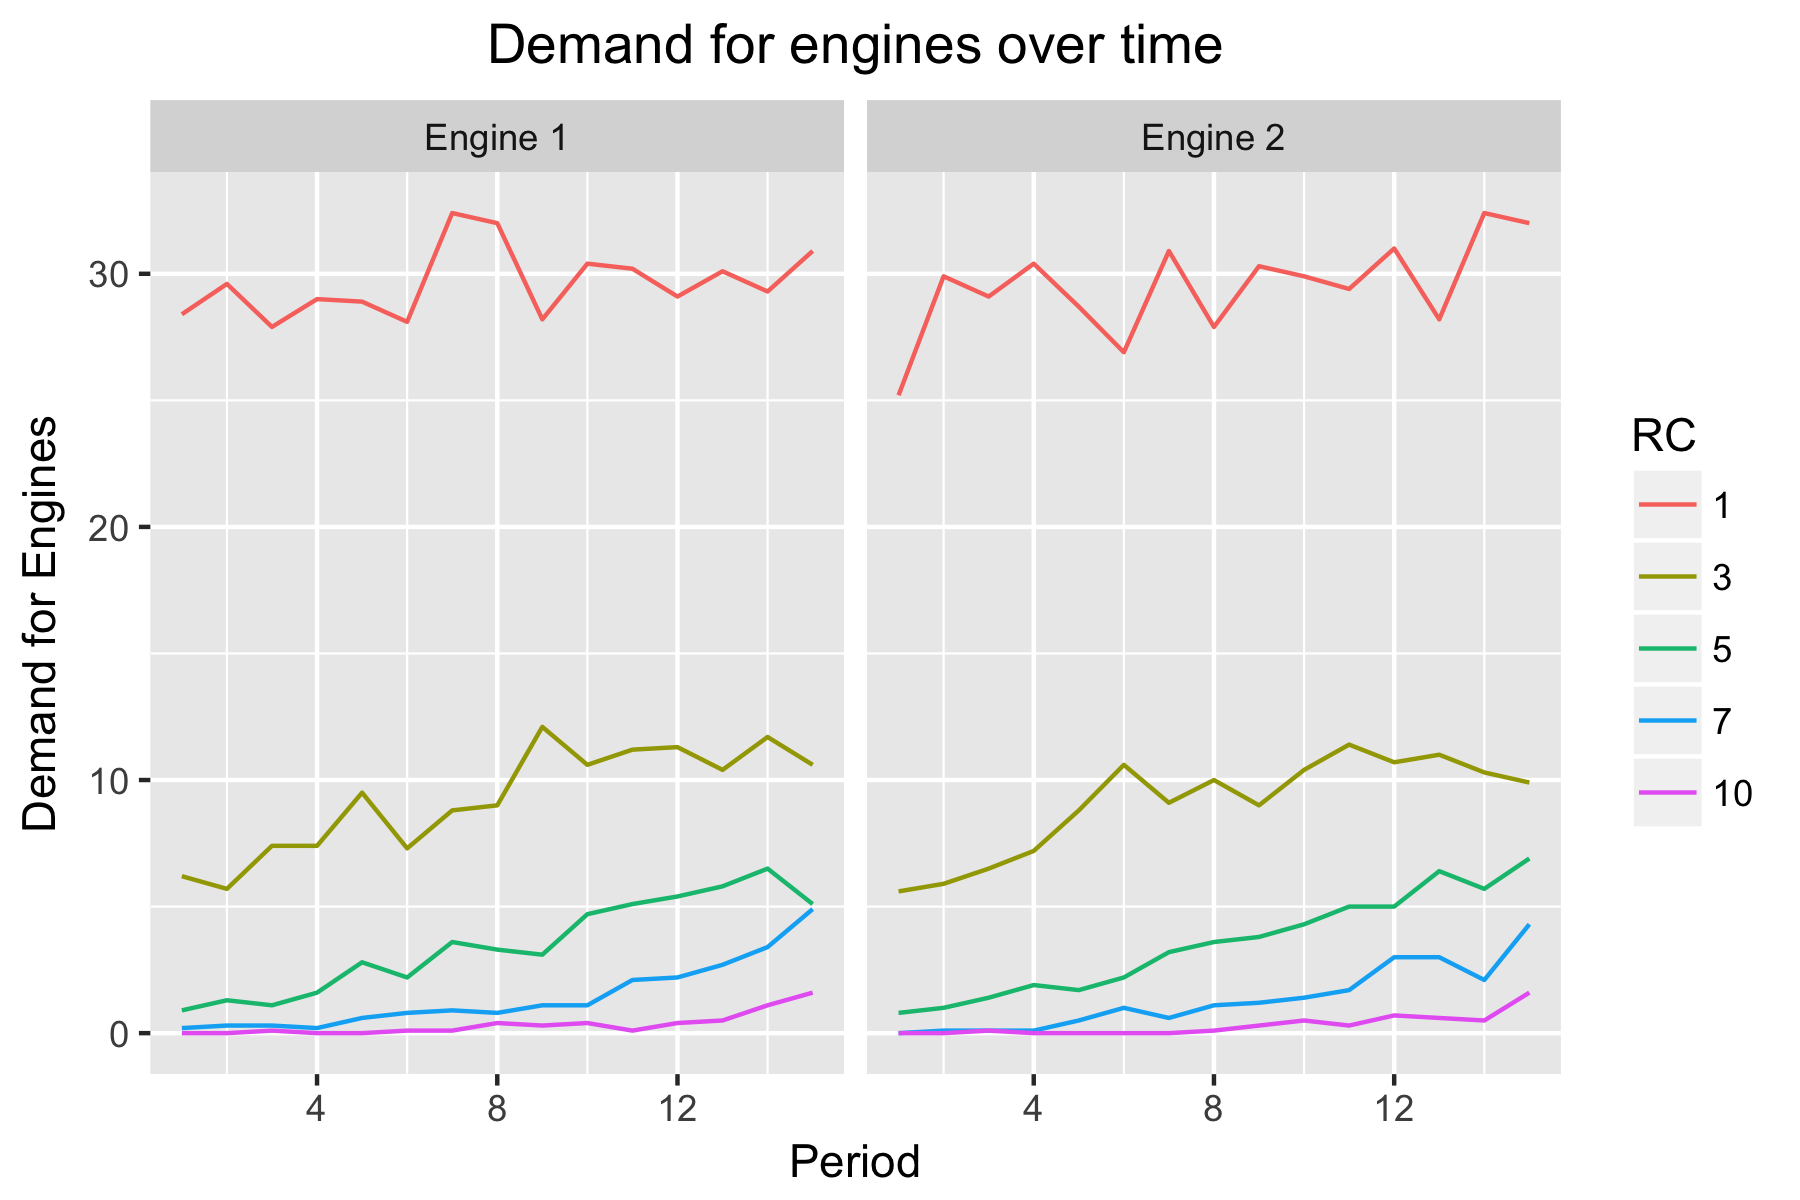
\includegraphics[scale=.25]{per_period_demand_plot.png}
\caption{The demand for engines across a fleet of 100 buses as a function of period (over the first 15 periods) for different values of RC. Unsurprisingly, when RC is lower, HZ is much more willing to change bus engines.}
\label{fig:time_demand_rc}
\end{figure}

\begin{figure}[ht!]
\centering
	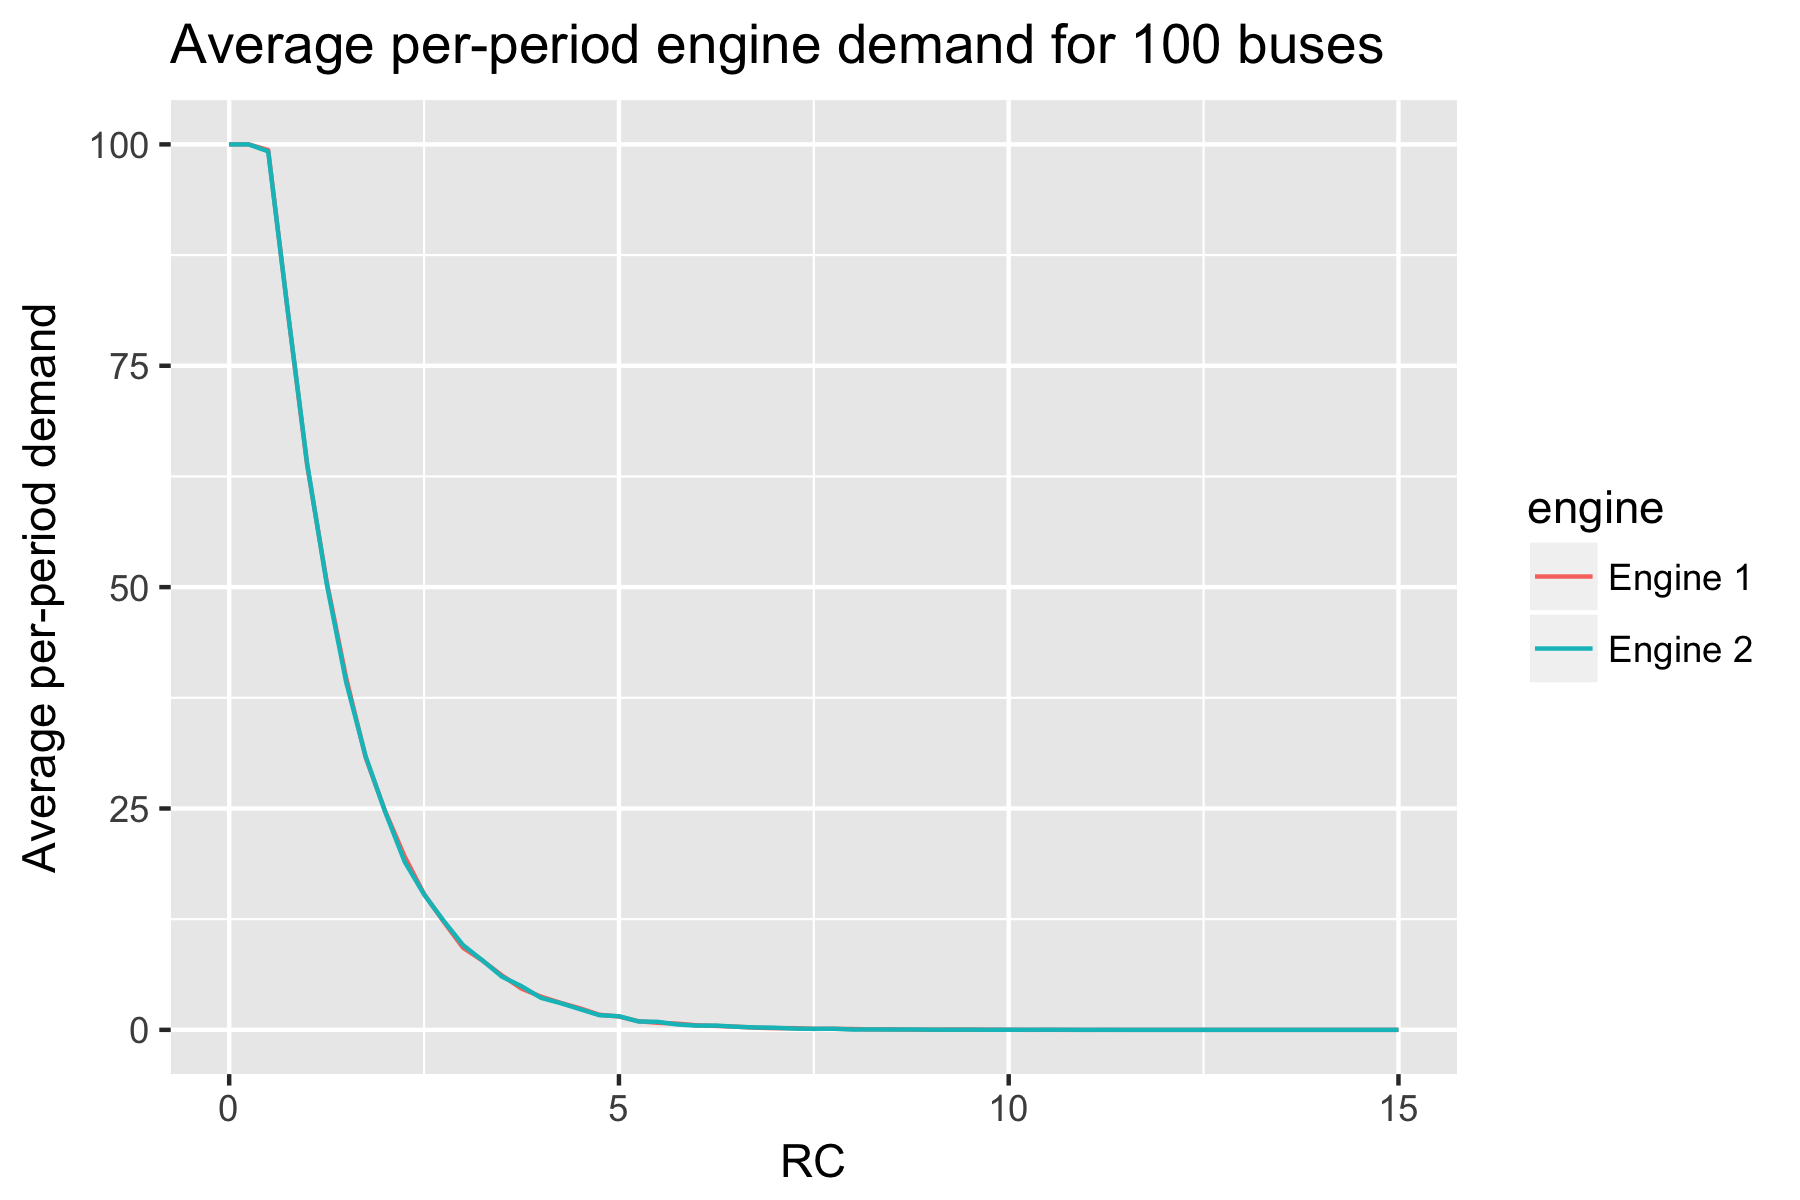
\includegraphics[scale=.25]{aggregate_demand_plot.png}
\caption{Aggregate per-period demand for new engines across a fleet of 100 buses as a function of RC. For engine 1, $\theta_1 = 0.05$. For engine 2, $\theta_1 = 0.02$.}
\label{fig:agg_demand_rc}
\end{figure}


We want to compute HZ's demand function for the two buses, which we will denote as engine 1 ($\theta_1 = 0.05, RC = 10$) and engine 2 ($\theta_1 = 0.02, RC = 20$) as a function of RC. In order to do so, we obtain conditional choice probability estimates, $\hat{\mathbb{P}}(i = 1 | x)$ by using the Rust \cite{rust1987optimal} method to iterate EV values. We use the Rust methodology because the Hotz and Miller \cite{hotz1993conditional} methodology depends on the observed conditional choice probabilities, which we know do \textit{not} correspond to the counterfactual engine 2.

With those conditional choice probability estimates for the two engines in hand, we run 1,000 simulations of a bus's state transitions (and HZ's corresponding engine replacement decisions) over the first 15 periods. This allows us to get an expected, per-bus demand for engines over the first 15 periods. In order to get the expected demand that HZ has for engines across all buses, we simply multiply this figure by 100. So the expected demand (as a function of period $t$) is:

\begin{equation}
D(t) = 100 \times \sum_{x_t} \hat{\mathbb{P}}(i = 1 | x = x_t) \hat{\mathbb{P}}(x = x_t | t)
\end{equation}

HZ's demand for engines as a function of the period, $t$ for a few values of RC can be found in Figure \ref{fig:time_demand_rc}. The average per-period demand for the two engines (averaged across 15 periods) for different values of RC can be found in Figure \ref{fig:agg_demand_rc}. it's worth noting that the demand curves for the two engines appear almost identical - there are only small differences (on the order of a tenths of an engine) between the two. This could be a true difference, or it could be simulation error. Although we're not sure why these demand curves are so similar, we have two hypotheses:

\begin{enumerate}
\item Our Rust EV estimates are highly sensitive to initialization. It's possible our estimates for engine 2 are not correct.
\item The increase in RC from engine 1 to engine 2 is almost perfectly offset by the decrease in $\theta_1$, creating two extremely similar demand curves.
\end{enumerate}

\item[(5)]

To determine the total value of the engines, assuming marginal cost $RC$, we can simply compute the total area to the right of a given $RC$ in a demand curve that looks like Figure \ref{fig:agg_demand_rc}. This area will give the total surplus that HZ gets from the engine in a given period.  In order to get a total value, we simply multiply this by the number of periods we want to consider. Mathematically, it is socially optimal to produce the more efficient engine if the total value is greater than the total cost:

\begin{equation}
V_{engine}(RC) - C(RC)= n \cdot \int_{RC}^{\infty} D_{engine}(p) dp - n\cdot RC \cdot D_{engine}(RC)- c > 0
\end{equation}

\noindent where $n=15$ is the number of periods and $D(p)$ is the amount of demand that HZ would have a given RC and $c$ is the fixed R\&D cost. Let's assume that $c$ is 0 for engine 1 (the status quo engine). Figure \ref{fig:value_plot} shows the value produced by both engines as a function of $RC$, assuming that $c = 0$. We can see here that, similarly to demand, the value produced by the two engines is very similar.

\begin{figure}[ht!]
\centering
	\includegraphics[scale=.25]{value_plot.png}
\caption{Value produced by the two different engines as a function of $RC$. We assume that $c = 0$ (i.e., R\&D costs are zero) for both engines. For engine 1, $\theta_1 = 0.05$. For engine 2, $\theta_1 = 0.02$.}
\label{fig:value_plot}
\end{figure}

Theoretically, the maximum justifiable development would be $value_2 - value_1$, if that quantity were positive (otherwise it is zero). For engine 1 at $RC = 10$, the total value is 2,447.1. For engine 2 at $RC = 20$, the total value is 0 (because our estimated demand is zero at $RC=20$). In light of this, there is no R\&D cost at which development of engine 2 would be justified. 

\end{itemize}

\end{itemize}

\newpage
\section*{Appendix: Code}

\mylisting[language=R]{./rust.R}

\bibliographystyle{plain}
\bibliography{pset4}
\end{document}
